%%%%%%%%%%%%%%%%%%%%%%%%%%%%%%%%%%%%%%%%%%%%%%%%%%%%%%%%%%%%
% Pedro Brandao's trial to get a template for thesis for students
% Used the upthesis from Fernando Silva (see upthesis).
% See also the packages file.
% 2014/07/07 First draft
% 2014/07/21
%  pbrandao: added the list of listings (it should produce portuguese name if
%           babel is set to portuguese, see packages.tex). Changed usepackage of babel
%           to be before input packages.tex to allow test

%
%%%%%%%%%%%%%%%%%%%%%%%%%%%%%%%%%%%%%%%%%%%%%%%%%%%%%%%%%%%%
% LTeX: language=portuguese

% makes all pages the height of the text on that page. No extra vertical space is added.
\raggedbottom
% setting it to report will remove the blank pages before each chapter
\documentclass[11pt,a4paper,twoside]{book}


%%%%%%%%%%%%%%%%%%%%%%%%%%%%%%%%%%%%%%%%%%%%%%%%%%%%%%%%%%%%
%%%   Packages that need to be configured for the thesis
%%%%%%%%%%%%%%%%%%%%%%%%%%%%%%%%%%%%%%%%%%%%%%%%%%%%%%%%%%%%

% Language settings
% use UKenglish for UK or leave blank for US English
% it will also change the names for some of the chapters (list of tables, figures, content,
\usepackage[UKenglish]{babel}
%\usepackage[portuguese]{babel}
% If you have multiple languages (as in this text) you can use both, leaving last the main one.
% Then you can use
% \begin{otherlanguage}{UKenglish}
% text in other language, UKEnglish in this case
% \end{otherlanguage}
%\usepackage[UKenglish,portuguese]{babel}

%%%%%%%%%%%%%%%%%%%%%%%%%%%%%%%%%%%%%%%%%%%%%%%%%%%%%%%%%%%%
%%%   Packages uses language definitions
% see file below for more packages and settings
%%%%%%%%%%%%%%%%%%%%%%%%%%%%%%%%%%%%%%%%%%%%%%%%%%%%%%%%%%%%
\usepackage{upthesis}


% the bibliography file
\addbibresource{refs.bib}


%% Definitions for acronyms
\newcommand*\acronymbiggest{DWARF} % defines the biggest Acronym used to define the column size



\usepackage[
%backref={section},
%pagebackref, % for getting references to the page where the citation is (in the biblio), note that biblatex above also has this
pdfpagelabels=false
]{hyperref}
\hypersetup{pdftitle={Using eBPF for Network Analysis}, %nao suporta acentos
   pdfkeywords ={bpf ebpf ieee mesh network analysis observation monitoring linux},
   pdfsubject = {assunto},
   bookmarksnumbered=true,
   pdfauthor ={Autor}, % see other options on manual (can be page) needs empty line on bibitem
   plainpages=false,
   pdfborder={0 0 0},
   colorlinks,%colorlinks=false,
   breaklinks=true,
	%hyperindex=true 	% Makes the page numbers of index entries into hyperlinks. Relays on unique page anchors (pageanchor)
% see for colors http://mirror.ctan.org/macros/latex/contrib/xcolor/xcolor.pdf
   linkcolor=Sepia, %MidnightBlue,% BlueViolet,%Sepia, % Color for normal internal links.
   %anchorcolor=black,% Color for anchor text.
   citecolor=RedViolet,% Color for bibliographical citations in text.
   %filecolor=cyan% Color for URLs which open local files.
   %menucolor=red% Color for Acrobat menu items.
   %runcolor=filecolor% Color for run links (launch annotations).
   urlcolor=NavyBlue% Color for linked URLs.
}
%use the same style for \url as the text
% from http://en.wikibooks.org/wiki/LaTeX/Hyperlinks#Customization
\urlstyle{same}

%%%------ added for comments
\usepackage{soulutf8}
\usepackage{color}

\DeclareRobustCommand{\hles}[1]{{\sethlcolor{cyan}\hl{ES: #1}}}
\DeclareRobustCommand{\hlrp}[1]{{\sethlcolor{orange}\hl{RP: #1}}}
% to make sure not comment is published, uncomment this
%\DeclareRobustCommand{\hles}[1]{}
%\DeclareRobustCommand{\hlrp}[1]{}
%%%------ end of added for comments

\addto\extrasUKenglish{
   \renewcommand\chapterautorefname{Chapter}
   \renewcommand\sectionautorefname{Section}
   \renewcommand\subsectionautorefname{Subsection}
}

\begin{document}

\title{eBPF for Mesh Network Monitoring}
%% The following is not currently being used.
% Part of the coverp in upthesis.sty
% \submitionplace{Tese submetida à Faculdade de Ciências da \\
%   Universidade do Porto para obtenção do grau de Mestre \\
%   em Ciência de Computadores}
% \author{Nome do autor}
% \department{Departamento de Ciência de Computadores \\ Faculdade de
%   Ciências da Universidade do Porto}
% \submitdate{Setembro 2015}

\beforepreface%

\prefacesection{Sworn Statement}

I, Carlos Tiago Gomes Pinto, born in 00/00/0000, resident in PLACE, phone number
000000000, of Portuguese nationality, bearer of Identification Card 00000000,
enrolled in the Master Degree Network and Information Systems Engineering at the
Faculty of Sciences of the University of Porto hereby declare, in accordance
with the provisions of paragraph a) of Article 14 of the Code of Ethical Conduct
of the University of Porto, that the content of this dissertation reflects
perspectives, research work and my own interpretations at the time of its
submission.

By submitting this dissertation, I also declare that it contains the results of
my own research work and contributions that have not been previously submitted
to this or any other institution.

I further declare that all references to other authors fully comply with the
rules of attribution and are referenced in the text by citation and identified
in the bibliographic references section. This dissertation does not include any
content whose reproduction is protected by copyright laws.

I am aware that the practice of plagiarism and self-plagiarism constitute a form
of academic offence.

Carlos Tiago Gomes Pinto

30/09/2022


\prefacesection{Abstract}

Being able to monitor the changes in a network is an important part of
experimentation and troubleshooting in the investigation field. In this work we
explore eBPF, a technology available in the Linux kernel that can be used not
only for monitoring, but also for the creation of monitoring tools, as well as
the different libraries and frameworks available to help with eBPF usage.

Using eBPF, we develop a tool for monitoring the creation, modification, and
removal of paths in \ac{IEEE} 802.11s mesh networks in Linux, for use with
wireless interfaces that use the softMAC implementation included in the kernel,
mac80211. The tool captures events that change paths and associate them with the
packets that triggered the changes, whenever applicable. It provides an
interactive graphical user interface that gathers information collected in the
different nodes and presents it to the user. Along with the development, we also
present the tests and work that was done in the exploration of eBPF and the
mac80211 subsystem of the Linux kernel.


\prefacesection{Resumo}

A capacidade de monitorizar mudanças numa rede de computadores é uma parte
importante da experimentação e resolução de problemas na área da investigação.
Neste trabalho exploramos o eBPF, uma tecnologia disponível no kernel Linux que
pode não só ser usada para monitorização, mas também para a criação de
ferramentas de monitorização, e as diferentes bibliotecas e \textit{frameworks}
disponíveis para ajudar com o uso do eBPF.

Usando eBPF, criamos uma ferramenta para monitorizar a criação, modificação, e
remoção de caminhos em redes \textit{mesh} \ac{IEEE} 802.11s no Linux, para uso
com interfaces sem fios que usam a implementação softMAC incluída no kernel,
mac80211. A ferramenta captura eventos que alteram caminhos e associa-os com os
pacotes que provocaram as mudanças, sempre que aplicável. Fornece também uma
interface gráfica que junta a informação gerada nos diferentes nós e apresenta-a
ao utilizador. Em conjunto com o desenvolvimento, também apresentamos os testes
e trabalho realizados na exploração do eBPF e do subsistema mac80211 do kernel
Linux.


\prefacesection{Acknowledgements}

I want to thank first and foremost my advisors Rui Prior and Eduardo Soares for
the tremendous help they have given me throughout these last twelve months. I
would also like to thank the Instituto de Telecomunicações (UIDB/50008/2020) for
hosting this work.

I also want to thank my parents for the support they have given me throughout my
whole life, and my friends for the joyous times we spent together.


% \dedicationpage{Dedico a \ldots}

% end of thesis preamble
\afterpreface%

%% main tex here
%% By putting the chapter names here, one can just comment the content in the chapters
%% and produce a pdf with the correct chapter number.
%% If you want further configurability you can use subfiles package
%% https://www.ctan.org/pkg/subfiles


%\chapter{Introdução}\label{chap:intro}
\chapter{Introduction}\label{chap:intro}

Monitoring and observability have always been important aspects in the field of
computer systems. They can be found everywhere, being used to determine the
performance and health of systems by administrators, used by programmers in the
form of debuggers, and even in research, to analyse new technologies and verify
that they are working as expected.

Several monitoring tools have been created over the years for all kinds of
purposes and hardware, but as components and software become more advanced,
these tools end up having to be replaced or updated. One of these newer tools
that has been gaining popularity in the last few years is eBPF.

eBPF is a technology that started out as the \ac{BPF}, which was a tool for
writing efficient packet filters. It has since been improved, having received
new capabilities, and also updated in order to take advantage of newer hardware,
transforming into eBPF. eBPF allows users to write programs that run on certain
events of the Linux kernel, allowing not only for monitoring of its internals,
but also enhancing its capabilities without the need to use kernel modules, all
of this while still ensuring the security and stability of the kernel. Because
eBPF can not only be used to access the internals of a system, but also
intercept the packets that system sends and receives, eBPF can be used to
monitor a whole network of systems.

One example of how eBPF can be used, is to monitor a network of systems in
\ac{IEEE} 802.11s wireless mesh networks, by probing the functions in the Linux
kernel related to these mesh networks in each of the systems in said networks.


\section{Aims and Objectives}

The main objective of this work will be to study eBPF, seeing what it can and
can not do, and determining how it can be used for network observability in
experiments, particularly in \ac{IEEE} 802.11s networks. We will then proceed
with the development of a tool that uses eBPF to demonstrate the type of
monitoring applications that can be built with this technology, revealing the
exploratory work that was done in order to realise this tool.


\section{Organization}

This thesis will start with the background in \autoref{chap:stat}, where we will
go over \ac{IEEE} 802.11 and \ac{IEEE} 802.11s mesh networks, as well as what
eBPF is in more detail, and explaining the different tools that can used to take
advantage of this technology.

Next, \autoref{chap:expl} will cover the exploratory part of this work, where we
mention the steps we took to understand how the Linux kernel's implementation of
the data link layer for \ac{IEEE} 802.11 networks (mac80211) deals with
\ac{IEEE} 802.11s mesh networks, mentioning some of the tests used for this
purpose and to get some experience with writing eBPF programs.

In \autoref{chap:devel} we talk about the development of the program that was
written to serve as an example of a tool that uses eBPF for network monitoring,
going over each section of its code. We also introduce the companion program
that was created to view the results generated by the main program.

Some of the tests that were used during development are explained in detail in
\autoref{chap:tests}, where we analyse what was learned from them, and the
decisions taken based on their results, including the final test that was
performed with the finished program running in real hardware.

Finally, in \autoref{chap:conc} we take a look at what we managed to accomplish,
and the limitations we had to settle for. We also mention parts of our programs
that could be improved upon, together with possible solutions.

There is no ``State of the Art'' chapter as there was no state of the art
surrounding the use of eBPF for monitoring \ac{IEEE} 802.11s mesh networks at
the start of this work.


%\chapter{Background}\label{chap:back}
\chapter{Background}\label{chap:stat}

This chapter will introduce the \ac{IEEE} 802.11 network technical standard
together with \ac{IEEE} 802.11s mesh networks, as well as explain eBPF in
detail, and reference the major libraries and frameworks used to facilitate the
development of eBPF programs.


\section{Mesh Networks}

The \ac{IEEE} 802.11 is a standard that is part of the \ac{IEEE} 802 group of
technical standards, and specifies the \ac{MAC} and \ac{PHY} protocols used to
implement communication of computers in a \ac{WLAN}. The standard has evolved
over the years since its first publication in 1997, and the revision published
in 2012 incorporated several amendments, one of which was 802.11s, which
introduced a definition for the creation of wireless mesh networks in a
\ac{WLAN}~\cite{ieee80211}.

A \ac{IEEE} 802.11s wireless mesh network is a network of devices, called mesh
stations, that are interconnected to each other, as shown in
\autoref{fig:meshnet}, with these connections being formed and destroyed
dynamically by the stations themselves, without the need for a central station
to manage these connections. Links are established when stations are able to
communicate directly, and data that needs to travel a large distance is fed
through the connections of the mesh network in a series of hops, allowing for
the communication of stations that are too far apart to communicate directly.
Some of the stations in a mesh network can also act as portals to other
networks, such as the Internet, providing, in this example, Internet access to
the whole network. These are referred to as mesh portals~\cite{meshopor}.

\begin{figure}[htb]
   \centering
   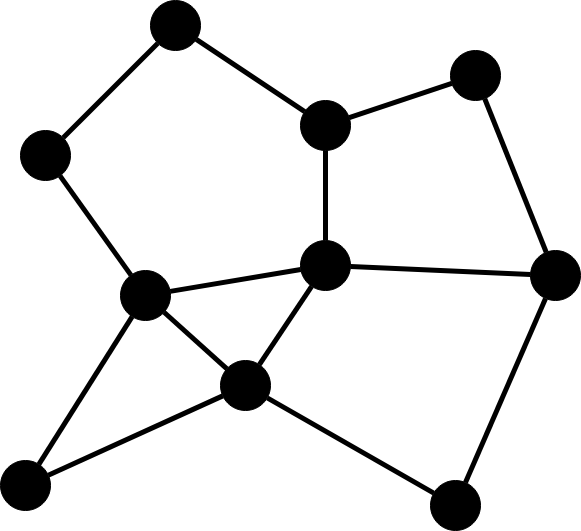
\includegraphics[scale=.4]{meshnet}
   \caption{Example of an \ac{IEEE} 802.11s mesh network}\label{fig:meshnet}
\end{figure}

The layer 2 routing protocol defined by \ac{IEEE} 802.11s that is used to create
and destroy these links is known as \ac{HWMP}~\cite{ieee80211}. In this
protocol, each station discovers other stations and manages a table of its
existing connections through a usage of the peer link management protocol, where
a station transmits beacons (frames with information about a network), and other
listening stations that want to become members of the same mesh network reply to
these transmissions. The table used to store these connections keeps not only
the direct connections the station has, but also the connections to stations
that are farther away, keeping an additional \textbf{nexthop} value, which holds
the address of the station that is directly connected to the source that
provides the best path to the destination, as seen in \autoref{fig:nexthop}. As
the name suggests, this protocol is hybrid, and it consists of two main
components. A proactive protocol, which is a tree-based hierarchical routing
protocol, and a reactive protocol, which is a modification of the
\ac{AODV}~\cite{aodv} routing protocol~\cite{ieee80211s}.

The proactive protocol works by having a station act as a designated root node,
and is only used when stations want to communicate with the root node or with
devices outside the mesh network~\cite{hwmpproa,hwmpperf}. When stations need to
communicate with other stations in the mesh network, the reactive protocol is
used. In this protocol, when a station needs to communicate with another, it
broadcasts a \textbf{Path Request} message with the \ac{MAC} address of the
destination. Intermediary stations rebroadcast this message while keeping
information from the transmitter of the message, in order to reach back with the
response. When the destination receives it, it updates its path to the source
and sends back a \textbf{Path Reply} in unicast~\cite{hwmpperf}.

\begin{figure}[htb]
   \centering
   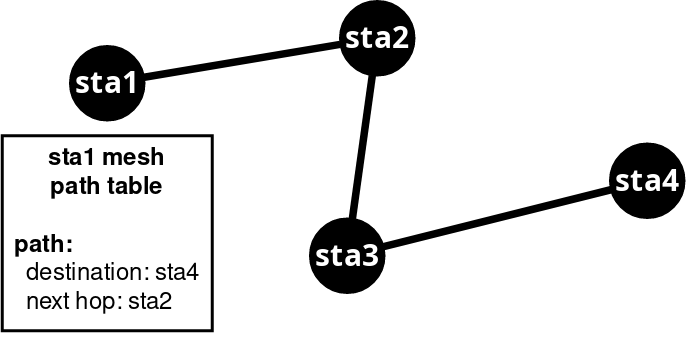
\includegraphics[scale=.4]{nexthop}
   \caption{Example of a mesh path}\label{fig:nexthop}
\end{figure}

In the Linux kernel's implementation of the data link layer for \ac{IEEE}
802.11s mesh networks, the connections between stations are known as
\textbf{mesh paths}, and the table where each system tracks these connections is
referred to as the \textbf{mesh path table}.


\section{eBPF}

The \ac{BPF} started out, as the name would suggest, as a packet filtering tool,
used only to accept or reject packets. This tool was created because the
existing packet filters were inefficient, having been developed for older
hardware. \ac{BPF} not only changed the design of the filter evaluator used,
replacing the stack-based one used by the original Unix packet filter with a
register-based evaluator, but it also changed the buffering strategy, resulting
in improved performance, among other things~\cite{bpf}.

\ac{BPF} filters packets using a directed acyclic control flow graph, where
nodes represent packet field predicates, and edges are control transfers. So,
for example, nodes would have checks in the form of "ether.type=IP", and edges
would be either a "yes" or a "no", with the flow going along the path of the
correct result. This approach is quite efficient, as it allows a \ac{BPF}
program to create a single flow graph that passes through several predicates,
having to parse each packet a single time, and ends in either a ``True'' or
``False'', deciding whether a packet should be processed or not, as seen in the
example in \autoref{fig:bpfprog}~\cite{bpf}. These filters can be written by
system administrators, and then run inside the Linux kernel, which allows
\ac{BPF} to check the packets before they are processed by the kernel.

\begin{figure}[htb]
   \centering
   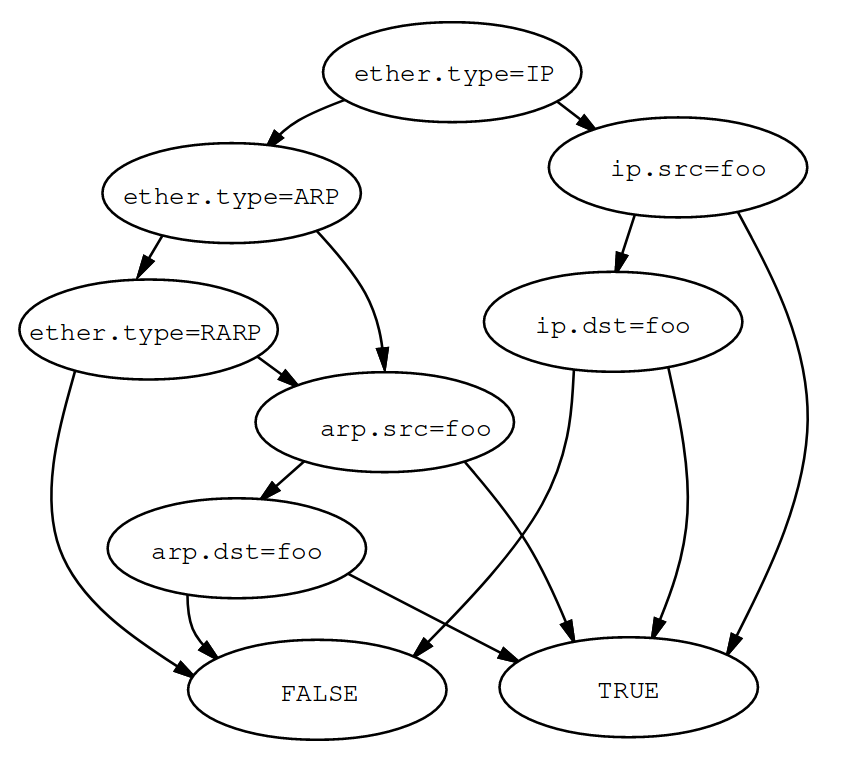
\includegraphics[scale=.3]{bpfprog}
   \caption{Example of a BPF program (Source:~\cite{bpf})}\label{fig:bpfprog}
\end{figure}

Seeing the potential of being able to write programs to run inside the kernel,
Alexei Starovoitov decided to improve \ac{BPF}, creating eBPF~\cite{alexei},
which used to be an acronym for ``extended BPF'', although that is no longer the
case~\cite{ebpfio}. Instead of simple flow-chart-like programs that can only be
used for packet filtering, eBPF now allows users to write more complex programs
that can involve arithmetic, structures, and pointers.

eBPF programs are executed on events, like function calls and network events,
through the use of, for example, \textbf{probes}, which are programs inserted
dynamically at the beginning or end of functions, which can be seen in
\autoref{fig:syscall}, with \textbf{kprobes} being used for functions inside the
kernel, and \textbf{uprobes} for functions in user-space, as well as
\textbf{tracepoints}, which are static points already present in the kernel
introduced by the kernel developers. These programs are loaded into the kernel
with the \texttt{bpf} system call and then pass through a verifier that ensures
that they are safe to run and do not get stuck in loops, checking if there are
any unreachable instructions, infinite loops, or instructions that harm the
system. Naturally, the verifier introduces some limitations to eBPF programs,
such as a limited number of instructions per eBPF program (Linux version 5.2
increased this number from 4096 to one million~\cite{sizelimit}), disallowing
conditional loops, and requiring root privileges for most programs~\cite{lwm}.
Finally, these programs are passed onto a \ac{JIT} compiler that optimizes their
performance by translating the code into machine specific instructions. Also,
because eBPF is part of the Linux kernel, there is no need for external modules
to be installed to run these programs~\cite{ebpfio}.


\begin{figure}[htb]
   \centering
   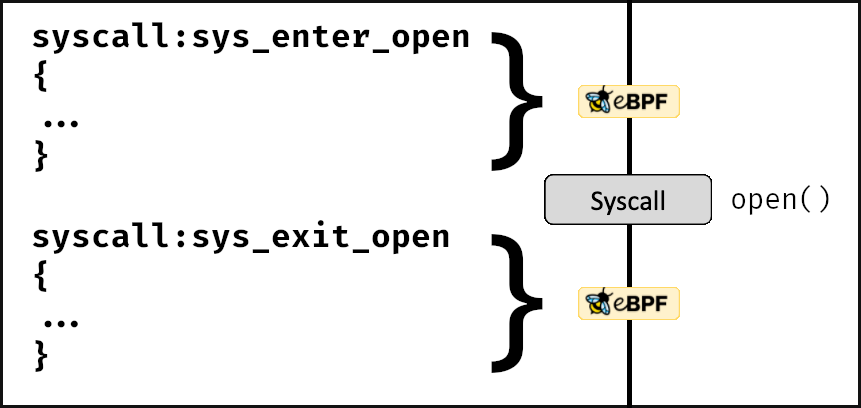
\includegraphics[scale=.35]{syscall}
   \caption{Example of eBPF tracepoints}\label{fig:syscall}
\end{figure}

eBPF also introduces mechanisms to help with development. Probes have already
been mentioned, but it also provides BPF maps, which allow programs to save data
temporarily in kernel-space, enabling sharing of information across probes and
to user-spaced~\cite{lwm}.

Not only that, but eBPF can also be used to write \ac{XDP} programs. \ac{XDP} is
a framework that allows for processing packets at the lowest possible level,
even before the kernel itself can process them. Some network cards even support
using \ac{XDP} in the controller itself, allowing for super fast processing of
packets. This, however, has limitations as well, since the programs are written
in a restricted variant of C, because they need to be translated into eBPF
byte-code, and \ac{XDP} can only be used in packet reception~\cite{xdp}.

eBPF has become an important tool in the last few years, especially in the area
of networks, having been used for discovery of dependencies in network
services~\cite{ebpfeg1}, taking advantage of its small performance overhead, as
well as monitoring traffic in Open vSwitches~\cite{ebpfeg2}, proving to be a
better choice against other monitoring solutions thanks to its code verifier,
which ensures that buggy eBPF code will not crash or otherwise severely
interfere with a system.


\section{BCC}

The \ac{BCC} is a toolkit with the purpose of allowing the creation of eBPF
programs more easily, with front-ends in both Lua and Python. This tool allows
for easier development of eBPF programs, as it abstracts the use of the \ac{BPF}
system call, replacing this with C-like code, which is then loaded into the
system with calls from a Python or Lua program. The toolkit is well documented,
and it also comes with some pre-made programs, which serve as examples of useful
eBPF programs~\cite{gregg,bcc}.

The ease of use comes at a cost, however, as \ac{BCC} embeds the LLVM toolchain
to compile programs, which leads to heavy processor and memory usage on
compilation~\cite{pingcap,contain}. This can become a problem since \ac{BCC}
compiles programs every time they are run. Not only that, but \ac{BCC} also
requires the system to have the kernel header packages installed, which not only
occupies extra space on the system to hold these
packages~\cite{pingcap,contain}, but can also be problematic, especially when
working with multiple Linux distributions, where the kernel header packages'
content can be different, which is exactly one of the problems we faced in
\autoref{sect:mac802}.

BCC used to be the primary choice for development of complex eBPF programs, but
it is now considered deprecated, with newer programs using libbpf together with
\ac{CO-RE}~\cite{toolsfuture}.


\section{bpftrace}

IO Visor, the project behind \ac{BCC}, has also introduced bpftrace, which is a
high-level language for tracing the Linux kernel that uses eBPF~\cite{bpftrace}.
Unlike \ac{BCC}, it is not a library, so no extra code is needed to run
programs. The user can simply write their bpftrace program and execute it
directly with the \texttt{bpftrace} command. However, it does not have an API
that allows for manipulation of data outside bpftrace. Also, like \ac{BCC},
bpftrace needs the kernel header packages for structure and other type
definitions~\cite{bpftrace}.

Due to being less verbose than \ac{BCC}, bpftrace is much easier to work with,
but because of its lack of API, which only allows to send information to the
standard output, it becomes useful only for programs that do not need to send
data to user-space. Still, if data needs to sent to user-space, bpftrace is
still useful for small tests and to quickly find all the available probes and
tracepoints through the usage of its \texttt{-l} flag, which lists all probes.


\section{perf}

perf is a Linux command used to analyse the Linux kernel's performance. perf
provides several subcommands that can record events, count the number of events
in a given timeframe, see events in real time, etc~\cite{perf}. perf was
originally created before eBPF, but it now uses it for tracing with tracepoints
and probes~\cite{greggperf}, and eBPF itself uses perf, for example, to send
data from BPF maps to user-space using perf buffers~\cite{perfring}.

perf is very similar to bpftrace, and like it, it is most suitable for smaller
scripts instead of big applications, suffering from the same disadvantages as
bpftrace.


\section{libbpf}

libbpf is a library written in C/C++ designed to allow loading and interacting
with eBPF programs~\cite{libbpf}. It is considered an alternative to \ac{BCC},
but with many advantages over it. libbpf abstracts many aspects of eBPF, just
like \ac{BCC}, but, unlike \ac{BCC}, which compiles the eBPF programs at
runtime, libbpf allows programs to be compiled into eBPF
bytecode~\cite{libbpf,contain}, eliminating the need of several dependencies on
the system in which the programs are being executed. Not only that, but libbpf
doesn't rely on kernel headers, instead using a header file that contains
multiple kernel structure definitions and types, eliminating the need for kernel
headers to be installed on the system~\cite{contain}. The drawback is that it is
not as well documented as \ac{BCC}, having almost only examples to serve as aid
in development.


\subsection{CO-RE}

\ac{CO-RE} is an approach implemented by libbpf that allows the creation of
portable eBPF programs, meaning that programs only need to be compiled once, and
can then be deployed across multiple systems, working even if these systems
differ in architecture and kernel version~\cite{coreref,fbslide}. This is
possible because of the \ac{BTF}. \ac{BTF} is a format that encodes debug
information, akin to \ac{DWARF}, but in a more compact and efficient manner, and
is used to provide information like structure offsets, which can then be used by
\ac{CO-RE} to relocate the eBPF bytecode as needed by the kernel version being
used~\cite{core}. This means that the kernel needs to be compiled with support
for \ac{BTF}. Thankfully, because \ac{BTF} support only amounts to about 1.5
megabytes in increase to the kernel image, most distributions already compile
their kernels for x86 architectures with the support~\cite{toolsfuture}.
Similarly to \ac{BCC}, a program needs to be created in order to load eBPF
programs, but \ac{CO-RE} also requires a file containing the structures and type
definitions used in the kernel to be generated (although this only needs to be
done once)~\cite{bootstrap}.

The problem with \ac{CO-RE} is pretty much the same as libbpf: it is not well
documented, and most of its documentation consists of a few blog posts made by
its main developer. The blog posts are actually quite well written, but they
only touch on the general uses of elements from \ac{CO-RE} with a few examples.
For more specific questions a developer might have, they are not very helpful.

Although libbpf and \ac{CO-RE} are recent technologies, they are used by big
companies like Facebook (where \ac{CO-RE} was created)~\cite{fbslide}, as well
as in projects for monitoring networks of Kubernetes clusters~\cite{kuber} and
security of Linux-based containers~\cite{sec}.


%\chapter{Estado da Arte}\label{chap:stat}
%\include{chap-soa}

%\chapter{Exploração}\label{chap:expl}
\chapter{Exploration}\label{chap:expl}

This chapter will go over the exploratory part of this work, discussing
experiments and analyses that were done in order to understand the functionality
of eBPF and how the network stack and mac80211 subsystem in the Linux kernel
work.


\section{Analysis of the mac80211 Subsystem}\label{sect:mac802}

The general idea for the tool that was to be developed was something that would
record the activity of a network and then display the changes that happened in
that network in a timeline. Alongside those events, we would have the packets
that caused them, so that the user could inspect those packets. But we still
needed to get to grips with eBPF because we had no prior experience with it.


\subsection{Exploration of the Network Stack}

We decided to begin by analysing the Linux source code using the Elixir Cross
Referencer~\cite{elixir}, and wrote small scripts with \textbf{bpftrace} to
better understand how the many components of eBPF, like maps and probes, could
be used to accomplish our objective, as well as to find the limits of this
technology. An example of one of these scripts was one that calculated the time
it took to send a \ac{UDP} network packet via the \texttt{sendto} system call
until the data to be transmitted reached the network card.

We started by seeing how glibc (GNU C Library) version 2.34 called the
\texttt{sendto} system call of the Linux kernel (version 5.15), and from there
followed the function calls in the kernel's code until we reached the function
\texttt{\_\_netdev\_start\_xmit}, which sends the data to be transmitted to the
appropriate network driver. This part was somewhat difficult, as most functions
could diverge, and macros are used a lot. The path of functions we followed for
IPv4 \ac{UDP} packets is as follows:
\begin{itemize}
    \item \texttt{\_\_sys\_sendto}
    \item \texttt{sock\_sendmsg}
    \item \texttt{sock\_sendmsg\_nosec}
    \item \texttt{inet\_sendmsg}
    \item \texttt{udp\_sendmsg}
    \item \texttt{udp\_send\_skb}
    \item \texttt{ip\_send\_skb}
    \item \texttt{ip\_local\_out}
    \item \texttt{dst\_output}
    \item \texttt{ip\_output}
    \item \texttt{ip\_finish\_output}
    \item \texttt{\_\_ip\_finish\_output}
    \item \texttt{ip\_finish\_output2}
    \item \texttt{neigh\_output}
    \item \texttt{neigh\_hh\_output}
    \item \texttt{dev\_queue\_xmit}
    \item \texttt{\_\_dev\_queue\_xmit}
    \item \texttt{dev\_hard\_start\_xmit}
    \item \texttt{xmit\_one}
    \item \texttt{netdev\_start\_xmit}
    \item \texttt{\_\_netdev\_start\_xmit}
\end{itemize}
For the script to record the time taken, we decided to use the entry tracepoint
of the \texttt{sendto} system call to save the timestamp of the call, and put a
probe in \texttt{\_\_netdev\_start\_xmit} to calculate the time taken. However,
we ran into an error because this function is inlined, and thus can not be
probed. The last function that can be probed is \texttt{dev\_hard\_start\_xmit},
but we could also probe the exit tracepoint of the \texttt{sendto} system call.
We decided to probe both the function and the exit tracepoint, for both to
calculate the time. This way we would get two different times: the time it took
from the system call until it reached the \texttt{dev\_hard\_start\_xmit}
function, and the time it took for the whole system call to complete. The code
for this script can be seen in \autoref{app:timer}.


\subsection{Finding Relevant Mesh Network Functions}\label{subs:mesh}

We wanted to monitor \ac{IEEE} 802.11s mesh networks in particular, so we
decided to check the content of the mac80211 subsystem. We tried to find
resources that mentioned which functions were used to manipulate the system's
mesh path table, but all we found were links to the source code files, which we
already had. The only solution that seemed viable was to find out these
functions ourselves. We started by going through all the files that had ``mesh''
in their name in the mac80211 subsystem folder, saving the names of all of their
functions. We then wrote a basic \textbf{bpftrace} script that probed all of
these functions, printing their name if they were called. This way, whenever
something that had to do with mesh networking happened in the kernel, we would
see the names of the functions that were executed. This script was quite big,
but a snippet of it can be found in \autoref{app:calls}.


\subsection{Use of Emulation}

To test this script we just needed an \ac{IEEE} 802.11s mesh network. For this,
we opted to go with an emulated network instead of using real hardware to save
on time and to make testing simpler and more predictable (ability to remove
interference, adjustable antenna range, etc.). We used
mininet-wifi~\cite{mnwifi}, which had everything we needed, and even included
the setup for an example mesh network.

We quickly ran into an issue with mininet-wifi, however. The Linux distribution
we were using was not officially supported by mininet-wifi. Thankfully, the
network emulator had virtual machine images available for this type of
situation, but we had some trouble with the packages in the repositories of the
distribution used by the virtual machine. Not only was the version of
\textbf{bpftrace} available quite old, but the package of the kernel headers
provided, which were used to get structure definitions, only had the files from
the \textbf{include} directory of the kernel source code, contrary to the
distribution we were using, which had all header files. These issues were
preventing our scripts from running. To solve this, we decided to try to install
mininet-wifi manually in our system, despite it using a distribution that was
not officially supported. Although it required some manual dependency checking
and installing, the mininet-wifi installation worked without problems.


\subsection{Filtering Out Irrelevant Functions}

Having mininet-wifi up and running, we executed the script we had written and
noticed that quite a lot of functions were showing up. Analysing the content of
these functions, as well as their comments (if they had any), we noticed that
most of them could be ignored, as they performed actions that did not affect the
mesh path table. After removing the functions that are not relevant for
monitoring path changes, we ended up with two functions in our list:
\texttt{mesh\_path\_add}, which inserts a mesh path in the mesh path table, and
\texttt{mesh\_path\_assign\_nexthop}, which changes the \textbf{nexthop} value
of a given mesh path. We didn't see any paths being deleted, but, knowing this
was possible, we considered \texttt{mesh\_path\_del} as well.


\subsection{Choice of eBPF Framework}

With these functions in mind, we started developing our program. We had to make
a choice between using \ac{BCC} or \ac{CO-RE}. Although more complex and with
less documentation, we decided to try \ac{CO-RE}, using the libbpf-bootstrap
repository available. However, we quickly hit a wall. The example in the blog
posts made by the author of \ac{CO-RE} mentioned that the file containing the
structure and type definitions used in the kernel needed to be generated with
the \texttt{bpftool} command, using the \ac{BTF} file
\texttt{/sys/kernel/btf/vmlinux}. The command seemed to have worked at first,
but including the generated file in our program was resulting in the error of
unknown structures used. Not finding any mention of this issue anywhere, and
with all the examples available using the exact the same command, we decided to
switch to \ac{BCC} using Python. Because the kernel headers package provided by
the distribution we were using included all the header files of the Linux source
code, we had no problems of unknown structures using \ac{BCC}.


\subsection{Probing Packet Transmission and Reception}\label{subs:pkt}

The idea of our program was to retrieve the data of the mesh path that was
inserted, modified, or removed from a mesh path table, by probing the functions
that performed these actions, store that data in a BPF map, probe a tracepoint
at packet transmission/reception, load the data stored in the BPF map, add the
important part of the packet content to it, and send it to user-space to be
processed by the user-space portion. We had already found the functions used to
retrieve the details of paths that were involved in modifications performed in
the mesh path table, but we still needed a way to get the content of the packets
that caused these actions. Thanks to the previously mentioned test that was done
at the beginning with bpftrace, we found a couple of tracepoints inside the
\texttt{xmit\_one} function that provided access to the \texttt{sk\_buff}
structure that holds the contents of packets.

For packet reception however, the task was a bit harder. We found a tracepoint
that worked, but the issue was that, because we are dealing with packet
reception, this tracepoint is called before any calls to functions that modify
the mesh path table, and we need to delete the content that was stored in the
BPF map for threads that did not change the mesh path table so as not to cause
memory leaks. This issue can be visualised in the difference between
\autoref{fig:pkttx} and \autoref{fig:pktrx}. One way to solve this issue would
be to find another tracepoint or function to probe located after any change to
the mesh path table, to capture all executions that also passed through the
packet reception tracepoint in order to delete the content stored in the BPF map
that was not used. Unfortunately, we did not find any tracepoint of function we
could probe that met these requirements.

\begin{figure}[htb]
   \centering
   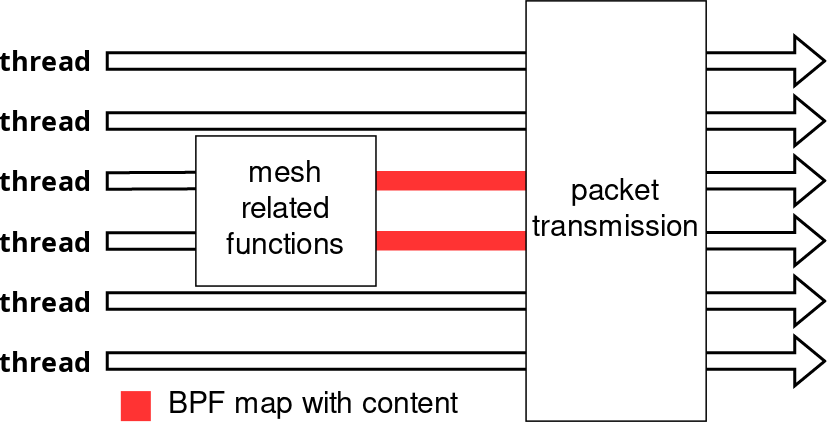
\includegraphics[scale=.4]{pktout}
   \caption{Use of BPF maps in packet transmission}\label{fig:pkttx}
\end{figure}

\begin{figure}[htb]
   \centering
   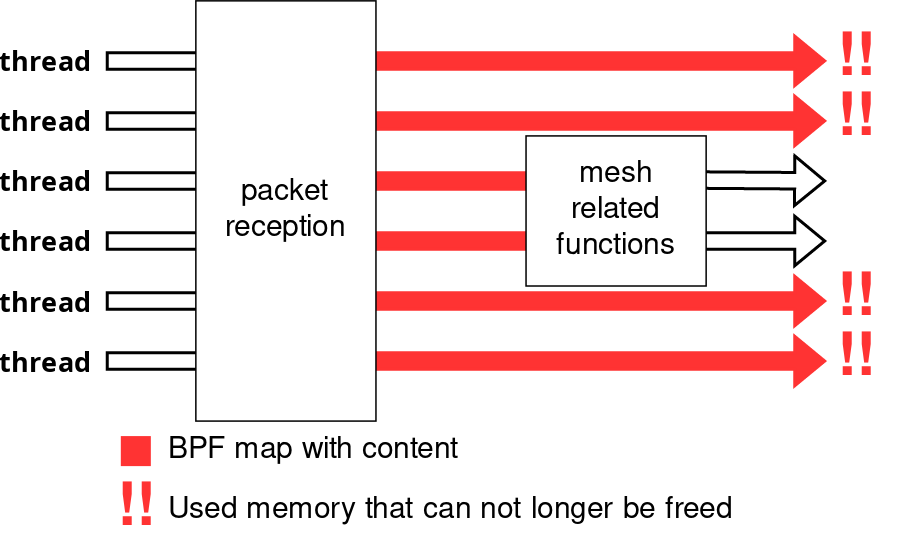
\includegraphics[scale=.4]{pktin}
   \caption{use of BPF maps in packet reception}\label{fig:pktrx}
\end{figure}

Because of this, we had to look for an alternative. We wrote a one-line script,
shown in \autoref{scr:stack}, that printed the call stack of kernel threads when
they passed through \texttt{mesh\_path\_add}, and found that the function
\texttt{ieee80211\_mesh\_rx\_queued\_mgmt} was called every time (except for
when mesh paths were added by packet transmission instead of reception), and it
had the \texttt{sk\_buff} structure in its arguments. After checking that this
function was called by a worker thread that executed
\texttt{ieee80211\_iface\_process\_skb} for every packet received, we decided to
use \texttt{ieee80211\_mesh\_rx\_queued\_mgmt}. We would still need to use two
probes, one at the function entry and another at the exit (because \ac{BCC}
can't get function arguments at the exit), but we could ensure that everything
that was written into the BPF map would later be removed.

\begin{sloppypar}
While looking for solutions to this problem, we also stumbled upon some
tracepoints that are called on commands from user-space that affected the mesh
path table, including insertion, modification, and deletion of mesh paths,
through the usage of the functions \texttt{ieee80211\_add\_mpath},
\texttt{ieee80211\_change\_mpath}, and \texttt{ieee80211\_del\_mpath}
respectively. Along with these tracepoints, there are also tracepoints at the
exit of these actions, used to retrieve the exit value of these functions.
Because these three functions all return \texttt{int}, we decided to add the
tracepoint \texttt{rdev\_return\_int} to our program to capture actions that
modify the mesh path table taken from the user-space.
\end{sloppypar}

\lstinputlisting[caption={Script to print the kernel stack},label=scr:stack,float=hb]{kstack.bpf}


\subsection{Capturing Relevant Packets}

At this point, we had the structure of the eBPF program pretty much set, but
there was still one thing we wanted to improve. We had access to the packets,
but we did not want to send their whole content to user-space, since we only
needed the content of the data link layer. While looking around the Linux
kernel, searching for how to access the fields that we would need, we found the
structure \texttt{ieee80211\_hdr} in the file
\texttt{include/linux/ieee80211.h}, and in the same file we found some functions
that led to examples of how the structure could be used, which was to cast the
\texttt{data} field of the \texttt{sk\_buff} as an \texttt{ieee80211\_hdr}
structure pointer.

We wrote a script that had a probe in the function \texttt{mesh\_path\_add}
where it added its thread ID in an BPF map, using the thread ID as the key as
well, and in the tracepoint \texttt{net:net\_dev\_xmit}, used in packet
transmission, it cast the \texttt{data} field of the \texttt{sk\_buff} structure
as an \texttt{ieee80211\_hdr} and printed all of its fields, if and only if the
BPF map had its thread ID stored. This resulted in the script printing the link
layer of packets that were being sent by threads that had inserted a mesh path
to the mesh path table earlier.

Running this script, we found that all the fields were correct except for the
address 1 field, which identifies the immediate receiver of the frame. Instead
of the address that was shown in the corresponding packet in Wireshark, the
field showed up as all zeros. After a bit of thinking, we realised that this
address shows as all zeros because the system that sent this packet only knew
the destination, but not the receiver, which could be the destination itself, or
any other device. Because this field would cause problems when comparing with
packets from the packet capture files, we decided to ignore addresses that show
as all zeros.


\subsection{Switch from BCC to CO-RE}\label{subs:switch}

After making sure the program worked in the emulated environment, it was time to
test it with real hardware. We started with a couple of computers with different
distributions and a Raspberry Pi. However, we ran into an issue we had already
faced before. Just like the distribution used by the mininet-wifi virtual
machine, most distributions' kernel header packages only include the header
files present in the \textbf{include} directory of the Linux source code,
meaning that some of the structures we were using were not available in the
Raspberry Pi, Ubuntu, Fedora, etc. We could solve this by copying the structures
we needed to our program, but these structures have other structures as fields,
which meant we needed to copy even more structures. Not only that, but we would
also need to be cautious of Linux updates changing the contents of these
structures. Another option would be to make the program depend on the Linux
source code, but not all distributions provide the source code as a package, and
this would also need to be updated along with the kernel itself. We ended up
trying to see if we could go back to using \ac{CO-RE}. After some time, we found
that \texttt{vmlinux} was not the only file in the \texttt{/sys/kernel/btf/}
folder. It includes plenty more files, one of them named \texttt{mac80211}. We
tried generating the file with the structure and type definitions using
\texttt{/sys/kernel/btf/mac80211}, and testing it, it worked without issues. As
a result, we decided to switch completely to \ac{CO-RE}.

We would need to switch from Python as we did not find a wrapper for it for
libbpf, which is needed to use \ac{CO-RE}. The languages we could use were
C/C++, Rust, or Go. We didn't want to deal with manual memory management if we
could, and with very little Go experience, so we decided to use Rust. Because of
how \ac{CO-RE} works, the eBPF portion also required some changes. One of the
biggest changes was the removal of the entry probe for
\texttt{ieee80211\_mesh\_rx\_queued\_mgmt}, because, unlike \ac{BCC}, \ac{CO-RE}
can access the arguments of a function at its exit. However, because arguments
can be pointers, as is the case for the argument with the packet content, the
content they point to at the exit can be different from the content they pointed
to at the entry. We did a few tests to check if the content of the packet
changed during the execution of the function and found that it never happened.
In the future, a more thorough assessment will be necessary to make sure that
this is always the case. Because using a single probe at the exit would simplify
the code structure, and we never saw the content of the packet change, we
decided to remove the probe at the beginning. The other main change was the
switch from probing \texttt{mesh\_path\_del} to \texttt{\_\_mesh\_path\_del}. We
did this because we were unable to retrieve the destination field of the path
from the arguments of \texttt{mesh\_path\_del}. We believe \ac{CO-RE} is capable
of this, but none of the examples provided helped in finding a solution. When
modifying the probe, we noticed that \texttt{\_\_mesh\_path\_del} was called
from other parts of the code as well, not just \texttt{mesh\_path\_del}, so we
added a few more probes to take those calls into consideration. These are
explained in detail in \autoref{subsec:ebpfcode}.

With these changes in place, the program started working on all the
distributions we were testing, but it still was not working in the Raspberry Pi.
Using the command \texttt{zgrep BTF /proc/config.gz}, we found that the kernel
being used in the Raspberry Pi was not built with \ac{BTF} support. Most
distributions build the kernel with this support for the x86 architecture, but
none of the distributions we tried for the Raspberry Pi offered the kernel with
\ac{BTF} support compiled in, so we tried to compile the kernel ourselves.
Unfortunately, that also failed without us understanding why. To prevent this
issue from blocking our progress, we decided to continue the development leaving
the Raspberry Pi aside for a later date.


\section{Event Capture and Packet Association}\label{sect:evepktasc}

As the main objective of the program was to show the user details about paths
that were added, modified, or removed from a system's mesh path table, along
with the respective packet that caused that action, we had to obtain this
information somehow.

Getting the details of paths was the easy part. As mentioned above, we probed
the functions that modified the mesh path table, and since they have a pointer
to the path structure in their arguments (except for \texttt{mesh\_path\_add}
which has other structures), we could take the information directly and store it
in a BPF map to send it to the user-space later.

The work required to get the packet content was somewhat more involved. In the
tests that we performed earlier, we noticed that whenever the mesh path table
was modified, functions related to packet transmission or reception were
executed, which meant that we could get the packet that caused the action by
following the thread's path. We set the probe and tracepoint used for packet
reception and transmission respectively mentioned earlier, and used the thread's
ID to check if a thread that was receiving/transmitting a packet had passed
through a function that modified the mesh path table earlier, and, if it did,
use that packet's content. Instead of sending the whole packet to the
user-space, we used a structure called \texttt{ieee80211\_hdr} to get just the
elements we needed in order to be able to unambiguously identify the packet.
We do this to keep the memory usage as low as possible and to minimise the
overhead of our eBPF programs. The fields we take from the packet are the
\textbf{Frame Control}, \textbf{Sequence Control}, and \textbf{QoS Control}
(when available) fields, as well as the three (four in some cases) MAC
addresses. We use the \textbf{Frame Control} to check the size of the data link
layer, as well as to check if the \textbf{QoS Control} field is included and if
there are three or four addresses. The \textbf{Sequence Control} is used to
differentiate packets that have all the other fields equal. According to section
10.3.2.14 of the \ac{IEEE} 802.11 standard~\cite{ieee80211}, only the first two
addresses of the MAC layer are needed to identify packets, along with the
\textbf{QoS Control} field, when it is present. Because we already had the
\textbf{Frame Control}, we thought we might as well use it for packet comparison
as well. We ended up not using the third and fourth addresses, but kept them as
well in case they would be needed in the future.


%\chapter{Desenho da Arquitetura}\label{chap:syst}
\chapter{Development}\label{chap:devel}

This chapter will cover the architecture of the tool that was developed to
realize the objective of this thesis. This tool captures the paths that were
created, modified, and deleted in a mesh network, and associates them with the
packets that caused these events.

The tool consists of two programs: a program that captures the events and saves
them in output files, which will be referred to as \textbf{service}, and a
program to view the captured events of several computers side-by-side, referred
to as \textbf{central}. The way this tool is meant to be used is summarized in
\autoref{fig:usage}.

\begin{figure}[htb]
   \centering
   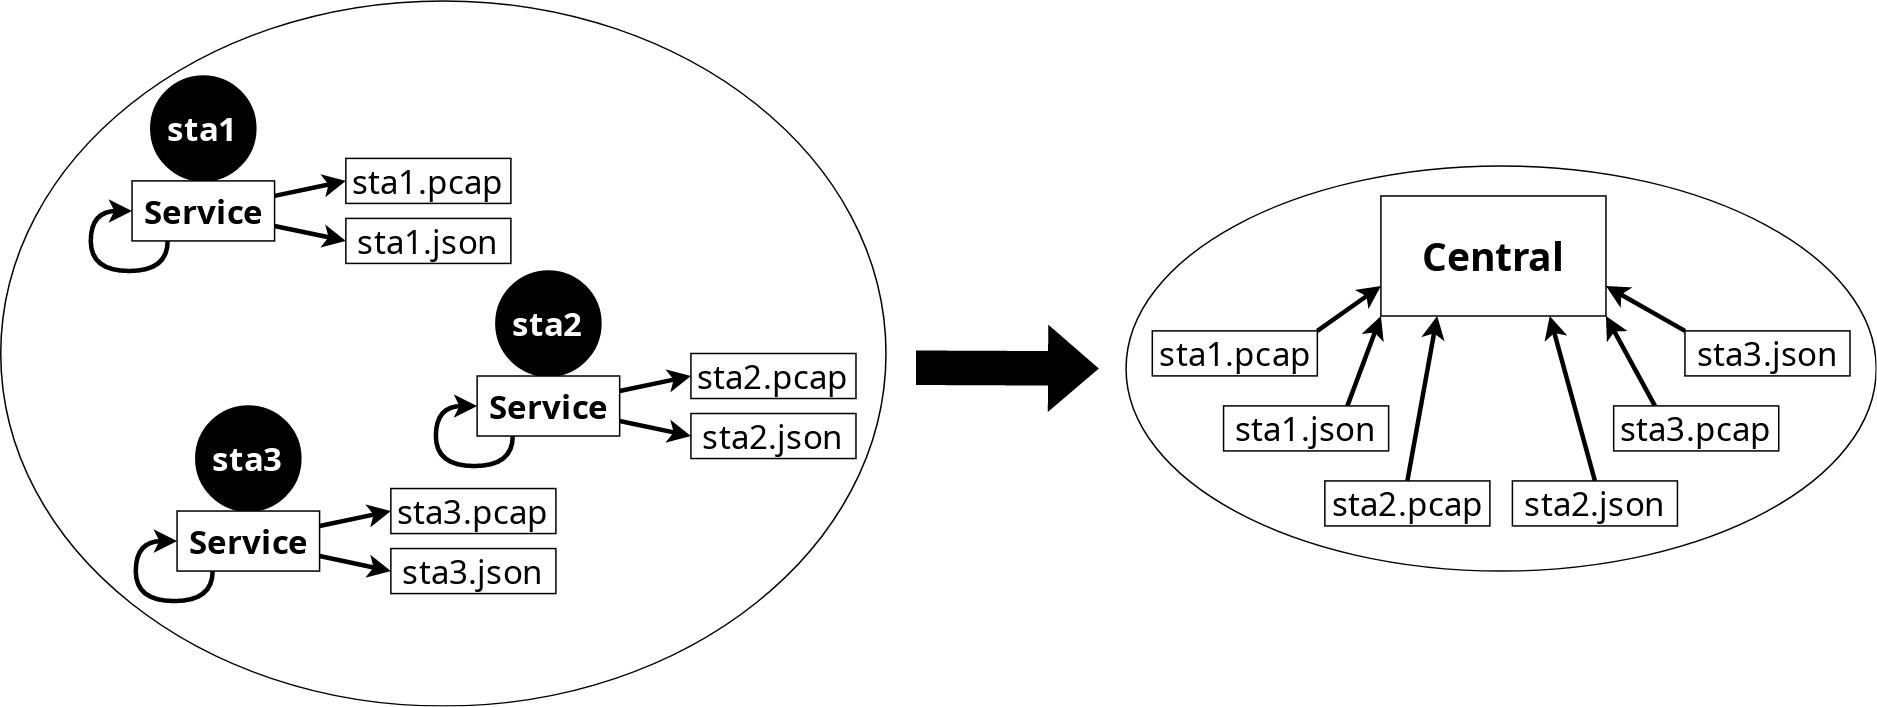
\includegraphics[scale=.225]{usage}
   \caption{Usage of the tool}\label{fig:usage}
\end{figure}


\section{Architecture of the Service}\label{sect:archser}

The \textbf{service} program can be divided into two parts. The eBPF part that
runs in the kernel-space and captures the events related to alterations in the
mesh path table, sending their details to user-space, and the Rust part that
runs in the user-space, receiving the data sent by the eBPF portion of the code,
while also capturing network packets at the same time in order to associate
packets to the actions performed in the system's mesh path table.

The \textbf{service} captures the events that alter the mesh path table and
network packets at the same time, saving them to output files, and when the user
sends a signal to stop, the program stops these captures. It starts by creating
the output files, a JSON file that stores a list of events and a network capture
file that stores packets, and then loads the eBPF code. Then, a new thread is
created whose sole purpose is to capture network packets. This new thread keeps
capturing packets and storing them in the appropriate output file in a loop that
only stops when the program receives a termination signal (one of
\texttt{SIGTERM}, \texttt{SIGQUIT}, or \texttt{SIGINT}).

Immediately after creating the packet capturing thread, the main thread goes
into a loop of its own doing the same thing, but instead of capturing packets,
it captures events sent by the eBPF code. This loop uses the same conditional
variable used by the packet capturing thread, so when one of the threads
receives a termination signal, both exit their respective loops.

After receiving a termination signal and leaving their loops, the packet
capturing thread stops, and the main thread continues. It then reads the
contents of both output files, creating a list of events and an iterator over
packets. The reason the program creates the output files at the start and writes
to them immediately, instead of creating these structures first and writing them
to the output files at the end, is to prevent the loss of data in case of a
crash, as well as to limit the memory usage of the program when it is run for a
long period of time.

With these two structures, the program goes over all the packets and events, and
checks which packets resulted in which events, storing this information in the
events themselves (this process is explained in more detail in
\autoref{subsec:relate}). Afterwards, it rewrites the output file for the
captured events with the newly modified events (including the packets each event
is related to), and terminates.


\subsection{eBPF Module}\label{subsec:ebpfcode}

The eBPF portion of the code is composed of nine probes. There are three probes
that detect if an alteration is made to the mesh path table, three to detect the
source of the action (if it was a packet reception or transmission that caused
the change in the mesh path table, or if it came from a command from
user-space), two for when a path is removed because it expired, and the last one
is for a special case which we will discuss later.

The three probes used to detect alterations in the mesh path table are in the
functions \texttt{mesh\_path\_add}, \texttt{mesh\_path\_assign\_nexthop}, and
\texttt{\_\_mesh\_path\_del}, the first two having been discussed in
\autoref{subs:mesh} and the last one in \autoref{subs:switch}. These are used to
gather information about the mesh path involved, including its destination,
nexthop, as well as the timestamp of the event and the MAC address and name of
the interface. The probe for \texttt{mesh\_path\_add} is the simplest, as it
only stores the information about the path that was added in a BPF map. In
another BPF map, the probe stores a value (which will be referred to as the
\textbf{situation} value) that indicates that the information stored in the
first BPF map came from a path addition to the mesh path table.
\autoref{fig:detai} shows in detail how this and the following probes use these
maps. The probe for \texttt{mesh\_path\_assign\_nexthop} is a bit more complex,
as this function is used both when a new path is added, and when an existing
path is altered, meaning that \texttt{mesh\_path\_add} can be called before it.
Because of this, this probe checks if there is a \textbf{situation} value
already present for the running thread in the BPF map, changing it to a new
value indicating if the situation is a new path being added or if it is an
existing path being modified. The information about the path is stored in the
appropriate BPF map if necessary. The relationship between these two probes can
be seen in \autoref{fig:addmod}. The last probe, in
\texttt{\_\_mesh\_path\_del}, detects the removal of paths from the mesh path
table, and if we ignore the possibility of paths being expired, it works just
like the probe for \texttt{mesh\_path\_add}. The case of a path being expired
will be explained shortly.

\begin{figure}[htb]
   \centering
   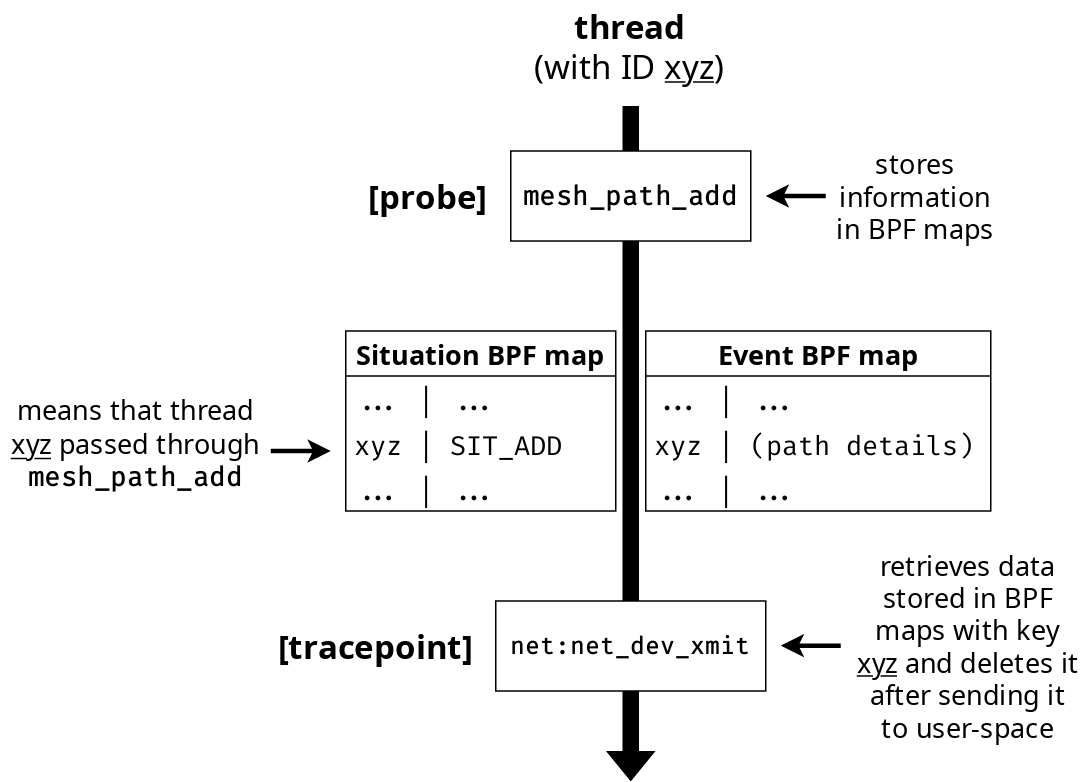
\includegraphics[scale=.375]{detail}
   \caption{Detail of BPF maps usage}\label{fig:detai}
\end{figure}

\begin{figure}[htb]
   \centering
   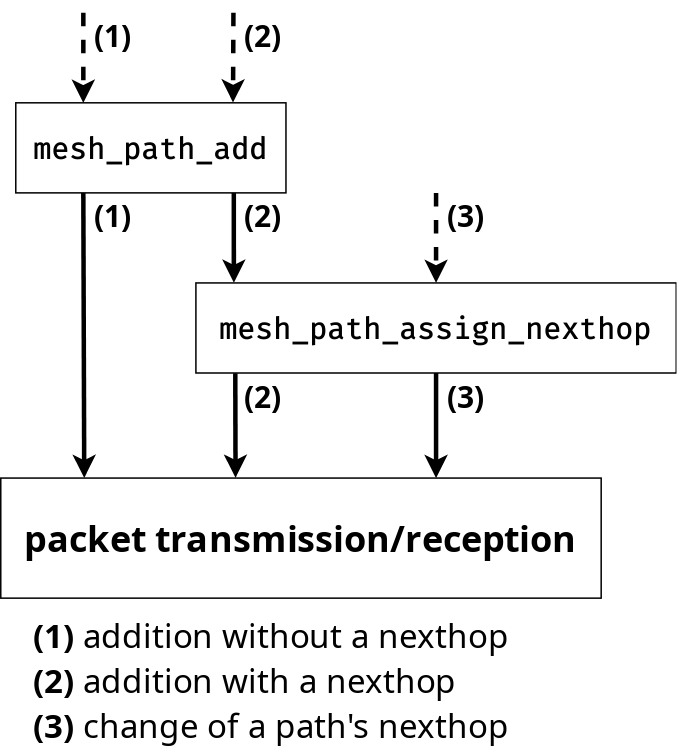
\includegraphics[scale=.35]{action}
   \caption{Probes for insertion and modification}\label{fig:addmod}
\end{figure}

For the next three probes, which are talked about in \autoref{subs:pkt}, two are
located in the tracepoints \texttt{net:net\_dev\_xmit} (packet transmission),
and \texttt{rdev\_return\_int} (command from user-space), and the third one is
in the function \texttt{ieee80211\_mesh\_rx\_queued\_mgmt} (packet reception).
These probes all work the same way. They take whatever is in the BPF maps, and
with the aid of the \textbf{situation} value, set the event's correct
\textbf{reason} field (which specifies the action taken on the mesh path table
and its source) and send the event to user-space to be received by the Rust
portion of the code, including the content of the link layer of the packet that
caused the event, if applicable.

There are also two probes at the entry and exit of the function
\texttt{mesh\_path\_expire}. The entry probe sets the \texttt{situation} value
in the proper BPF map, so that the probe at \texttt{\_\_mesh\_path\_del} sends
the event information directly to the user-space, while the exit probe simply
removes the data from the BPF maps, as it is not needed any more. The reason to
use two probes this way instead of having a single probe sending the data to
user-space directly (like the other three previously discussed), is because
\texttt{mesh\_path\_expire} calls \texttt{\_\_mesh\_path\_del} more than once.
Since only one event can be stored at a time per thread (because the threads'
IDs are being used as the keys in the BPF maps, and BPF maps do not allow the
usage of arrays of structures), only the information about the last path being
deleted would be sent to user-space instead of all paths. The way these probes
interact is demonstrated in \autoref{fig:delexp}.

\begin{figure}[htb]
   \centering
   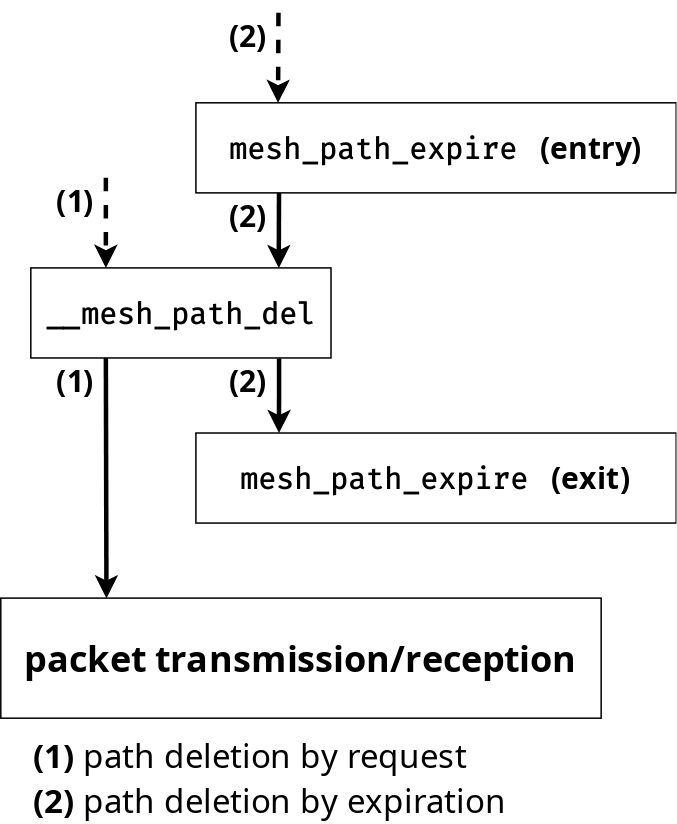
\includegraphics[scale=.35]{actiondel}
   \caption{Probes for deletion and expiration}\label{fig:delexp}
\end{figure}

Finally, there is also a probe in \texttt{mesh\_plink\_deactivate}, which is a
function that calls \texttt{\_\_mesh\_path\_del} indirectly. This probe is used
to ignore any calls to this function. The reason for this is that we were not
able to determine all the possible reasons for this function being called.
Packet transmission and reception would be captured, but some actions could be
missed. For example, we found that this function could be called by
\texttt{ieee80211\_sta\_expire}, and to capture this we would need more probes,
just like how probes for \texttt{mesh\_path\_expire} were required. Because we
found many functions calling \texttt{mesh\_plink\_deactivate}, and any of them
could end up requiring more probes, the time it would take to analyse all the
different possibilities would be too much, so we decided to ignore calls to this
function.


\subsection{Packet and Event Relation}\label{subsec:relate}

The packet/event relation section of the code is composed of two loops, one
inside the other. The program goes over every packet individually, and for each
one, it goes over every event that was captured. Even if an event gets matched
with a packet, the next packets will still check all events, including the ones
that matched with other packets earlier. This $O(n^2)$ algorithm is used, as
opposed to a more efficient one that would remove events as they are matched,
because of an issue that prevents us from obtaining the full content of a packet
in some events, where we have to ignore the missing content, which can lead to
an event matching more than one packet.

Because at the time of development a Rust library to access fields of network
packets did not exist, the program checks the raw data of the packets for the
fields manually in the array of bytes provided. It starts by making sure that
there are enough bytes to get all the data needed to compare with the details of
the event, and, if there are, compares the frame control, sequence control, and,
if applicable, \ac{QoS} control fields, as well as the address 1 and address 2
fields. As mentioned in \autoref{sect:mac802}, we noticed that in some events
the address 1 field obtained from the kernel-space was incorrect, it being the
address \texttt{00:00:00:00:00:00} instead of the expected value because the
computer that sends the packet does not know the \ac{MAC} address of the
receiver. We decided to ignore this field when it takes the aforementioned
value. We did not see this happen with the address 2 field, but do the same for
precaution.


\section{Architecture of the Central}\label{sect:archcen}

The \textbf{central} is a much simpler program than the \textbf{service}, as its
only goal is to display the events captured in a group of computers in a more
human-friendly way. Most of its code is for the \ac{GUI} logic.

The program takes a folder with the output files generated by the
\textbf{service} as an argument, and checks the file names, accepting only files
that end in \texttt{.json} and \texttt{.pcap}. For each pair of files that
contains the same stem, a structure called \texttt{Station} is created,
containing the list of events in the events file, and the name of the packet
capture file. After checking all files, a list of several \texttt{Station}
instances is returned.

The last step before displaying the events is to sort them in chronological
order. This is done by increasing the size of the list of events for each
station to have the capacity for all events in all the stations. Then, using
their timestamps, the events are ordered in such a way that, for each place in
the stations' lists, where one station has an event, all the others have an
empty element. This can be visualized in \autoref{fig:sort}. Although not very
efficient, it is the simplest method we could come up with to implement.

\begin{figure}[htb]
   \centering
   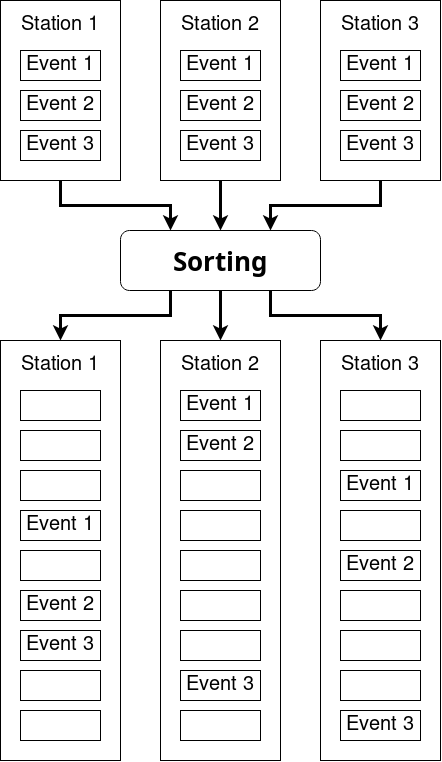
\includegraphics[scale=.4]{eventsort}
   \caption{Chronological sorting of events}\label{fig:sort}
\end{figure}

Finally, the \ac{GUI} is created, where the user can view all the events of all
of the stations side by side, and not only inspect the details of each event,
but also see the packets that caused those events in Wireshark with the press of
a button. \autoref{fig:hardtest} displays an example capture.

\begin{figure}[htb]
   \centering
   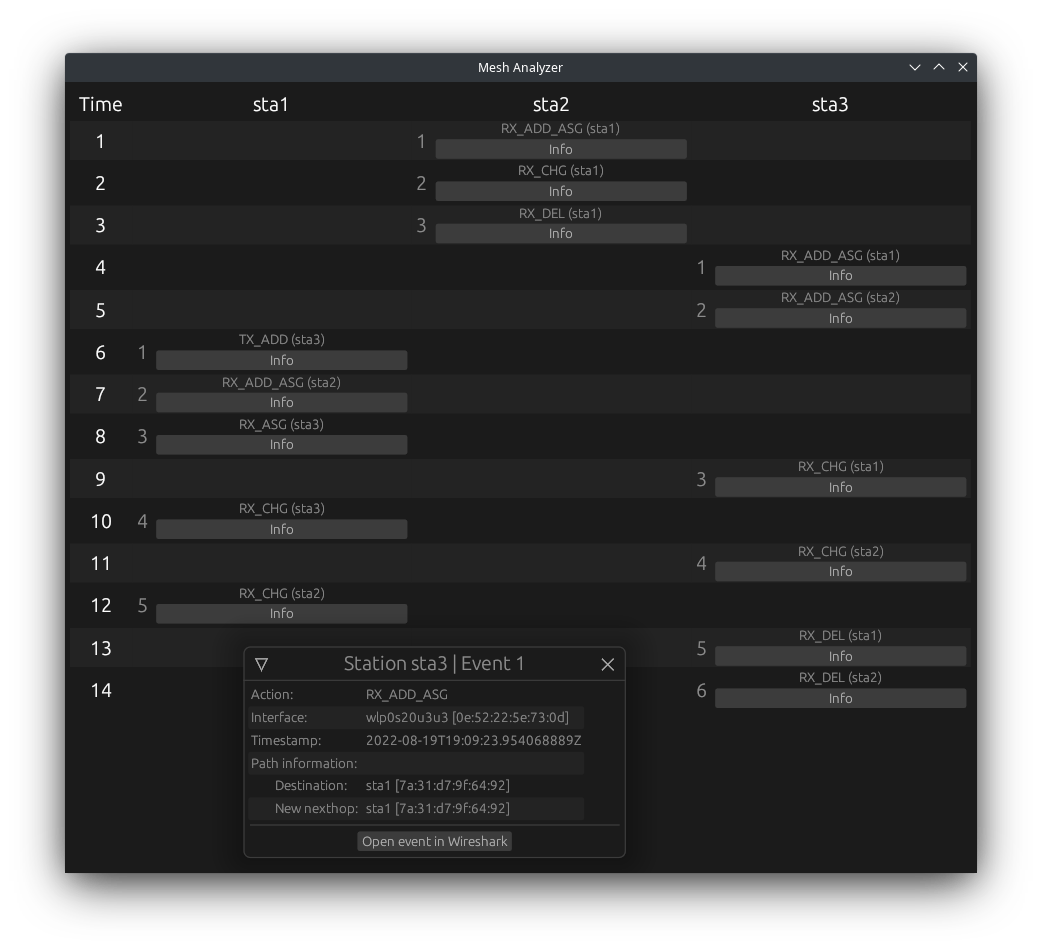
\includegraphics[scale=.575]{gui}
   \caption{\ac{GUI} interface}\label{fig:hardtest}
\end{figure}


%\chapter{Desenvolvimento}\label{chap:dese}
\chapter{Tests and Validation}\label{chap:tests}

Some of the tests made during the exploration have already been mentioned in
\autoref{chap:expl}, but here we will go over a couple of tests in detail that
were important in the development of our tool and verifying that it worked as
expected.

\section{Validation in Emulated Environment}

After developing the initial version of the full service program, one of the
tests we performed using mininet-wifi consisted of three stations (named sta1
sta2 and sta3), where sta1 and sta3 were too far apart from each other to
communicate directly, but both in range of sta2, as shown in
\autoref{fig:latetest}, and all of them without any paths in their mesh path
tables initially, pinging sta3 from sta1.

\begin{figure}[htb]
   \centering
   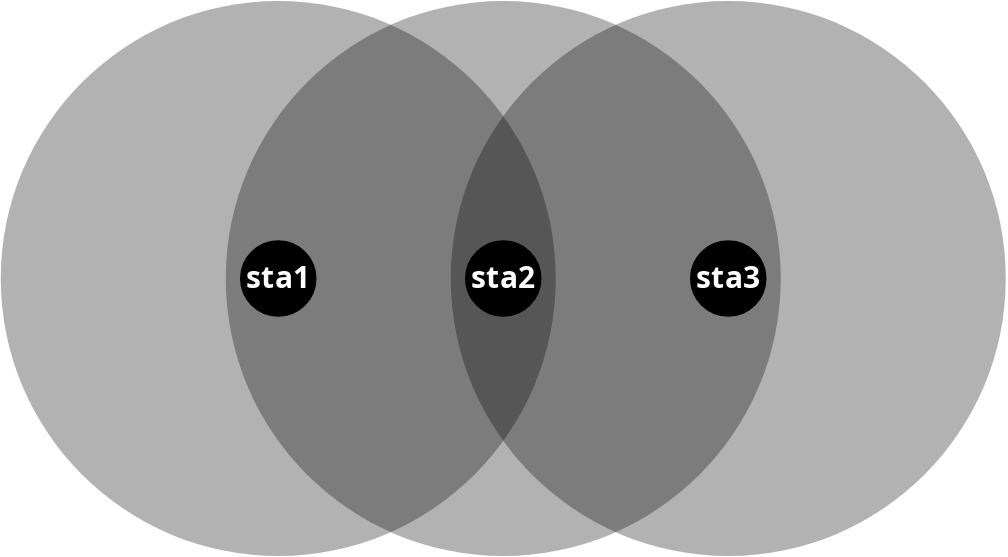
\includegraphics[scale=.3]{latetest}
   \caption{Test configuration used in mininet-wifi}\label{fig:latetest}
\end{figure}

We found that the first station to create and add a mesh path was sta3. Although
sta1 was the one that pinged sta3, it could not create a path yet because it did
not know the \ac{MAC} address of sta3. So sta1 only sends an \ac{ARP} request in
broadcast, which is then retransmitted by sta2, and after sta3 receives it, it
creates a path for sta1 (without the nexthop field filled in) when it sends its
\ac{ARP} response, highlighted in blue in \autoref{fig:capsta3}, which shows the
packet capture that was executed in sta3.

\begin{figure}[htb]
   \centering
   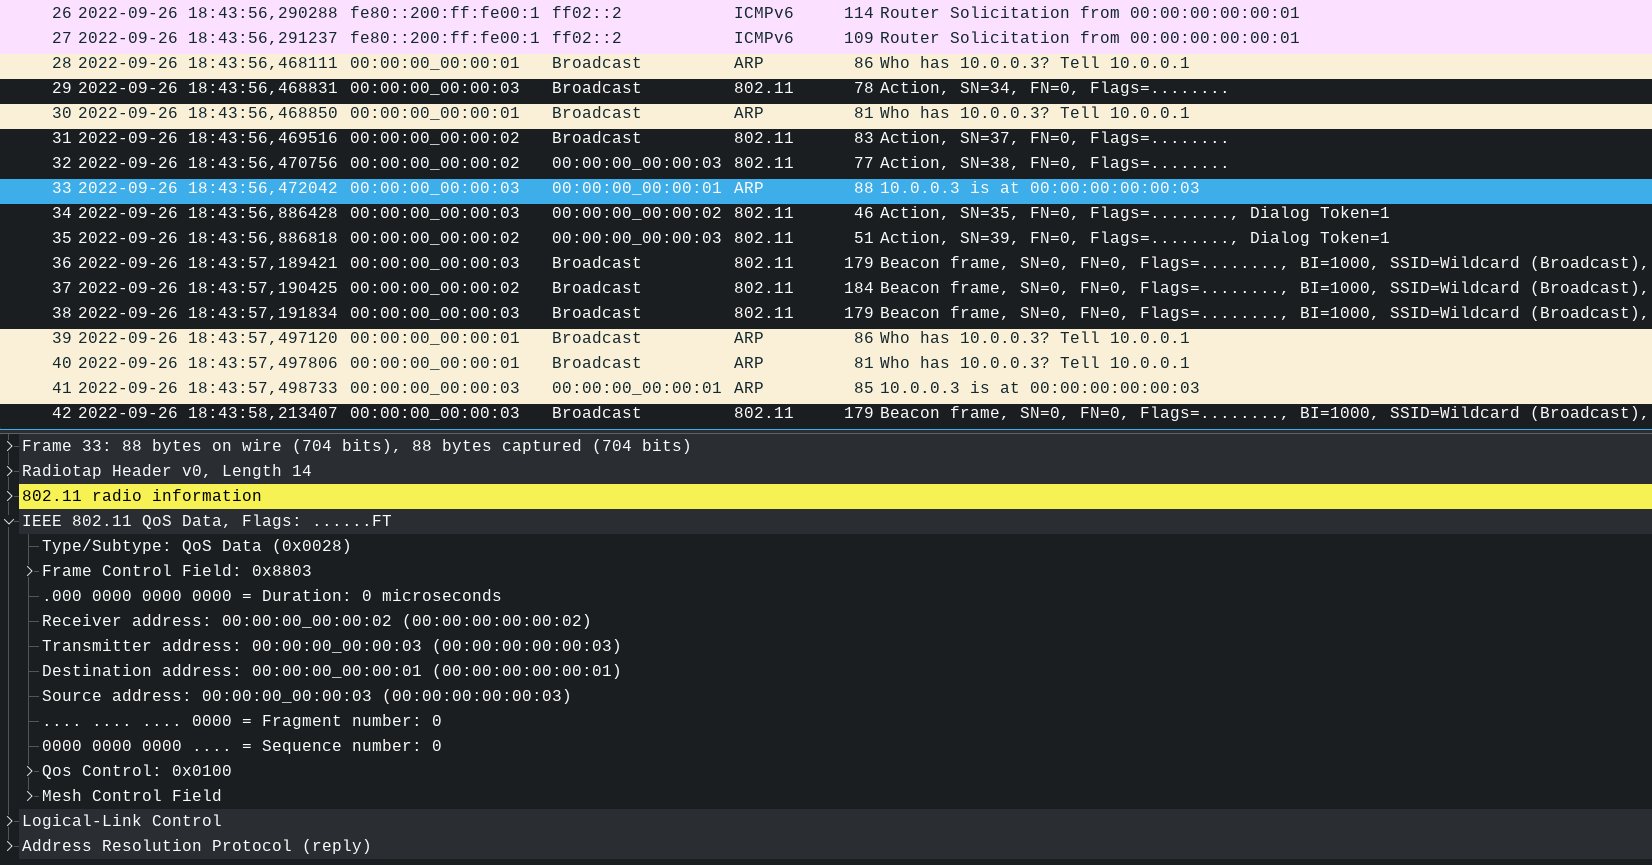
\includegraphics[scale=.35]{capsta3}
   \caption{\ac{ARP} response that caused a path to be added to the mesh path table}\label{fig:capsta3}
\end{figure}

Immediately after, sta2 creates a path to sta3 and retransmits the \ac{ARP}
response to sta1, which in turn receives the \ac{MAC} address of sta3 through
sta2, and creates its mesh paths, both for sta2 and sta3.


\section{Validation with Hardware Nodes}\label{sect:valid}

Because we spent most of our time in development testing with mininet-wifi, we
were only able to do a simple test with real hardware. We tried to replicate the
test mentioned in the previous section, placing sta1 and sta3 far away from each
other in the hopes that sta2 would be needed for the other two stations to
communicate, but the space we had was not enough, as can be seen in the results
displayed in \autoref{fig:hardtest}, which shows at the bottom details about the
first event captured in sta3, where a path was added with the destination and
the nexthop both set to sta1's \ac{MAC} address, meaning sta2 was not used for
communication between the two stations. Still, we can verify that the tool we
developed worked as expected, showing a mesh path being created and then deleted
in sta2 (most likely because it ended up not being used), and sta3 and sta1
creating mesh paths and settings their \textbf{nexthops} values.

We did notice some unexpected behaviour. For example, in event number 10, sta1
changed the \textbf{nexthop} field of its path to sta3 to the value it already
had previously, effectively not changing anything. The reason for this behaviour
was most likely a change to the path's sequence number, which is a field we do
not capture, but is maintained in the mesh path table entries.


%\chapter{Resultados e análise}\label{chap:results}
% \include{chap-results}

%\chapter{Conclusões}\label{chap:conc}
\chapter{Conclusion}\label{chap:conc}

Recalling what was said in \autoref{chap:intro}, the objectives of this thesis
were to explore how eBPF could be used for monitoring experiments in wireless
networks, and to create a program that would showcase this.

This work was very exploratory, as it was necessary to examine the code of the
Linux kernel which is not only very extensive but also very complex, study mesh
networks, as well as learn eBPF, all of which are fields where we had little to
no prior experience. Most of the documentation of eBPF and the tools and
frameworks around it assume some familiarity with the Linux source code, how it
works, and its most used structures, which was not the case for us.

As for the programs developed, we accomplished our objective, which was to
create a tool that could demonstrate how eBPF could be used in experiments of
wireless networks. Our service program can detect changes in the mesh path table
of several systems, and its output files can be then used in conjunction with
outputs from other systems to be analysed with the central program to get a
timeline of the activity in an entire mesh network.

It is worth mentioning that in our program we use probes as a necessity, which
are not as stable as tracepoints. This means that an update to the kernel that
changes the functions we probe could result in our program not working
correctly, and an update to fix these probes would be required.


\section{Future Work}

Although we were able to reach our objectives, we believe our programs could be
improved with more features and fixes to compromises that had to be made due to
the lack of time available. The following paragraphs contain some ideas and
possible solutions for the implementation.

The first one is the presence of the probe in the function
\texttt{mesh\_plink\_deactivate}. This probe ignores some actions that can
modify the mesh path table, so removing it would be an improvement. To remove
it, a deeper analysis of the functions that call
\texttt{mesh\_plink\_deactivate} would be needed, to take into account all the
possible call stacks.

One of the biggest issues we wanted to fix but could not for lack of time was
the way we sort all the events in the \textbf{central} program. We use the
timestamp captured along with the path information for sorting events, but since
the clocks of the several computers in a network being monitored will not be
perfectly synchronized, it is not a reliable metric. One way we think this could
be solved would be to use the ordering of packets instead, using two packet
capture files where one has a packet that causes a change to a mesh path table
being sent, and another has that same packet being received, and using that
packet as a basis for sorting events between the two stations where these
packets were captured. The timestamp of the events could additionally be used to
shift the events in a station that were not caused by a packet in relation to
the events in other stations, using the packet previously mentioned as a
reference point in time.

With hindsight, we can see that the decision to switch to a single probe at
packet reception when we switched from \ac{BCC} \ac{CO-RE} was not ideal. We did
it mostly because the code became shorter and much easier to comprehend. Still,
although we never detected it, there is a chance that some function could change
the content of a packet. If we had time we would revert to two probes, with the
entry probe inserting the important content of the packet to the BPF map, have
the probes at each action retrieve the information from the BPF map and
submitting it to user-space, and have the exit probe delete anything in the BPF
map for the cases where the thread did not alter the mesh path table.

Something that we think would be fun, but also help visualize bigger networks,
is to create a graph showing the mesh paths in each event. This would basically
be an easy-to-interpret timeline of the network. Being able to click on each
station to see the events that it captured, as well as each mesh path to see its
information, along with which packet (if applicable) caused it would be great as
well. Because the events already store the source, nexthop, and destination of
each path, this would only require updating the central program.

Another thing that would possibly help with bigger networks is a file that
contains the information of a whole network. Right now, the \textbf{central}
program takes the files of all the stations and sorts their events every time it
is executed. We never experienced a slow sorting process, with the program
always being opened almost immediately, but considering that our tests were
always quite short and involved at most three stations, it is possible that
bigger networks and longer tests would cause a slow-down. We think the
\textbf{central} program could have a flag that generates a file that contains
all the events of all stations already sorted, to be used in other runs, instead
of the original files.

Something that would be nice to have would be a way for the central program to
be able to retrieve the information gathered by the different nodes being
monitored automatically, instead of relying on manual file transfers from those
nodes.

The way we sort the events in the \textbf{central} program, although simple, is
not very efficient given that it increases the lists of events for each station,
filling them mostly with empty elements, which still occupy as much space in
memory as the structures for events. A better approach would be to use would be
preferable.

Something that could be improved is the fields of paths that the tool captures.
Currently, it captures only the destination and nexthop of paths, but other
fields can be captured, such as the metric value and the sequence number, as was
noted in the last paragraph of \autoref{sect:valid}.

One last thing that we think would help with analysis would be to show the time
between events. This would enable users to easily determine how much time has
passed between events, and could be implemented using the timestamps available
in the events.




%% references
%\renewcommand{\bibname}{Referências} % o babel portuguese coloca Bibliografia
% os meses do ficheiro bib poderão aparecer em inglês, caso se pretenda deve-se colocar o texto em português explicitamente no ficheiro bid
\cleardoublepage%
\phantomsection%
\begin{sloppypar}
\printbibliography[heading=bibintoc]%
\end{sloppypar}


%% appendix
\appendix
\chapter{Code Snippets}


\section{\texttt{sendto} Timing bpftrace Script}

\lstinputlisting[caption={bpftrace script},label=app:timer]{timer.bpf}


\section{Detect Mesh Network Function Calls}

\lstinputlisting[caption={bpftrace script},label=app:calls,float=hb]{calls.bpf}


%% bye
\end{document}
